\documentclass{homeworg} 
\usepackage{CJKutf8}
\usepackage{float}
\usepackage{multicol}
\usepackage{hyperref}
\usepackage{emoji}
\usepackage[mono=false]{libertinus}
\usepackage{luatexja-fontspec}

\usepackage{graphicx}
\usepackage{booktabs}
\usepackage{longtable}
\usepackage{tabu}
\usepackage{tcolorbox}

\newcommand{\file}[1]{{\color{blue}\texttt{#1}}}
\newcommand{\bc}[0]{\begin{CJK*}{UTF8}{bkai}}
\newcommand{\ec}[0]{\end{CJK*}}
\newcommand{\img}[1]{\includegraphics[width = 80pt]{#1}}
\newcommand{\hug}{\emoji{hugs}\phantom{x}}

\hypersetup{
    colorlinks=true,
    linkcolor=black,
    urlcolor=blue,
    citecolor=magenta
}
\title{}
\author{B08902134, 曾揚哲}

\begin{document}
\setemojifont{TwemojiMozilla}
\begin{center}
\def \coursename {ADL }
\def \hwn {2}
\Large \textbf{\coursename HW \hwn}    
\end{center}
\begin{flushright}
B08902134, 曾揚哲
\end{flushright}
\section{Data Processing}
\subsection{Tokenizer}
I use the \hug {\color{blue}\texttt{BertTokenizer} } pretrained with the model used for training. The tokenizer converts the word into tokens which could be recognized by \texttt{BERT} model. The tokenizer does the following:
\begin{enumerate}
    \item Convert each word into token represented by their respective unique ID, while division into subwords is used in western languages, Chinese tokens cannot be cut into subwords. 
    \item Add specific tokens such as \texttt{[CLS]},\texttt{[SEP]}  and  \texttt{[UNK]} to represent the classification token, separation token and the unknown words during pretrain phase of the tokenizer, respectively.
    \item Pad, truncate or split the context into lists in a task-oriented manner, which is done by the \hug tokenizer itself.
\end{enumerate}
\subsubsection{Context Selection}
Each data consist of a question and four relevant context, and they are tokenized in the following manner:\\
What I intended to do originally:\\\phantom{What}\texttt{[CLS]} tokenized question... \texttt{[SEP]} tokenized context 1... \texttt{[SEP]} \texttt{[PAD]}...\\
\phantom{What}\texttt{[CLS]} tokenized question... \texttt{[SEP]} tokenized context 2... \texttt{[SEP]} \texttt{[PAD]}...\\
\phantom{What}\texttt{[CLS]} tokenized question... \texttt{[SEP]} tokenized context 3... \texttt{[SEP]} \texttt{[PAD]}...\\
\phantom{What}\texttt{[CLS]} tokenized question... \texttt{[SEP]} tokenized context 4... \texttt{[SEP]} \texttt{[PAD]}...\\
But I write the code wrong so it is actually processed as:\\
\phantom{What} \texttt{[CLS]} tokenized question... \texttt{[space]} tokenized context 1... \texttt{[SEP]} \texttt{[PAD]}...\\\phantom{What}
\texttt{[CLS]} tokenized question... \texttt{[space]} tokenized context 2... \texttt{[SEP]} \texttt{[PAD]}...\\\phantom{What}
\texttt{[CLS]} tokenized question... \texttt{[space]} tokenized context 3... \texttt{[SEP]} \texttt{[PAD]}...\\\phantom{What}
\texttt{[CLS]} tokenized question... \texttt{[space]} tokenized context 4... \texttt{[SEP]} \texttt{[PAD]}...\\
But in the end it turns out to work (the performance is not bad?)!
\subsubsection{Question Answering}
Each data consist of a question and the selected context, and they are tokenized and truncated in the following manner:\\\phantom{What}
\texttt{[CLS]} tokenized question... \texttt{[SEP]} tokenized context part 1... \texttt{[SEP]}\\\phantom{What}
\texttt{[CLS]} tokenized question... \texttt{[SEP]} tokenized context part 2... \texttt{[SEP]}\\\phantom{What\texttt{[CLS]} tokenized question...}
$\vdots$\\\phantom{What}
\texttt{[CLS]} tokenized question... \texttt{[SEP]} tokenized context part n... \texttt{[SEP]} \texttt{[PAD]}...\\
I use the tokenizer with a \texttt{doc\_stride} of 128 tokens so that it could cover the longest answer, and only the context would be truncated, which could be done by passing \texttt{truncation="}{\color{red}\texttt{only\_second}}\texttt{"} to the \hug tokenizer.
\subsection{Answer Span}
\subsubsection{Preprocessing}
While the \hug tokenizer does the answer span processing for us, we could still inspect what it does for us. 
As mentioned in \textbf{1.1.2}, only the context would be truncated while a stride of it would be preserved in each vector. To elaborate on the detail, we here denote the maximum length of question and context pair, the length of the question, the length of the context part in each vector, and the padding length by $L$, $L_q$, $L_c$, $L_p$, respectively. Here, we assume that $L_q$ < \texttt{doc\_stride} and the whole question context pair is divided into $n$ vectors. Therefore, we have 
\begin{align*}
    L & = 1 + L_q + 1 + L_{c,i} + 1, 1 \leq i < n \\
    L & = 1 + L_q + 1 + L_{c,n} + 1 + L_p 
\end{align*}
For \texttt{doc\_stride} $t$, $L_{c,i - 1}[t:] = L_{c,i}[:t]$, $\forall 1 < i \leq n$. \\
To contain the largest question answer pair (ideally according to the training set), I set \texttt{doc\_stride} $= 128$.  Then we could find out that the each vector contains context of length $L_c' = L - 3 - L_q$, and hence the $i$-th vector will contain context$[i * (L_c' - \texttt{doc\_stride}): i * (L_c' - \texttt{doc\_stride}) + L_c' ]$. Given these information, it is easy to find the original start/end position in these vectors. Notice that this is easy because we are not requried to cut the context into subwords during tokenization because we are working on a Chinese dataset.
\subsubsection{Postprocessing}
After predicting the start/end positions in each vector, I take the \texttt{n\_best}$ = 20$ probabilties from the logits and exclude those positions that give 
\begin{itemize}
    \item answer not in the context
    \item ansewr with negative length, i.e., \verb|end_position| < \verb|start_position|
    \item answer that is too long, i.e. \verb|L_a| $> 30$
\end{itemize}
After finding the valid (\verb|start_position|, \verb|end_position|) pairs, I would return the answer who has the highest probabilties at the start and the end, theoretically multiplied, but I used summed assuming log are taken for logits score.\\
The predicted answer is then slightly modified as some brackets may not be closed after the prediction. For Chinese, I added (「,」, 《,》) to complete the bracket if the complement present. Moreover, the half-width comma (i.e. '\texttt{,}') was removed from the answer to prevent kaggle misintepreting it as the csv separator. With the bracket completion, the exact match on test dataset improved from 0.79746 to 0.80018 (pretrained model with best performance).
\newpage
\section{Modeling with BERTs and their variants}
Note: the reported metrics are recorded from the last epoch, while the result on kaggle was not necessarily inference with checkpoint from the last epoch. 
\subsection{Baseline Model}
\begin{enumerate}
    \item My model: \hug \texttt{bert-base-chinese} \\
    Configuration:
    \begin{itemize}
        \item Hidden size: 768
        \item Hidden Layers: 12
        \item Attention Heads: 12
        \item Intermediate Size: 3072
        \item \texttt{max\_len}: 512
        \item \texttt{doc\_stride}: 128
    \end{itemize}
    \item Performance\\
        \begin{tabular}{c|c|c|c|c}
            & Train Acc. / EM & Train Loss & Val. Acc. / EM & Val. Loss \\ 
            \hline Context Selection & 0.9988  & 0.0040 & 0.9629 & 0.1503 \\
            \hline Question Answering & 0.9769  & 0.0412 & 0.7988 & 0.9172
        \end{tabular}\vspace{10pt}\\ 
        Result on kaggle public test dataset:
        0.75406 (Strong Baseline: 0.75497)
    \item Loss Function: CrossEntropy Loss 
    \item Optimization:
    \begin{itemize}
        \item Algorithm: AdamW with \texttt{lr} $ = 2\times10^{-5}$ and weight decay $= 1 \times 10^{-6}$
        \item Learning Rate Scheduler: Cosine Annealing Scheduler with $1:9$ steps for warmup and training
    \end{itemize}
\end{enumerate}
\subsection{Model with best performance}
\begin{enumerate}
    \item My model: \hug \texttt{hfl/chinese-macbert-large} \\
    Configuration:
    \begin{itemize}
        \item Hidden size: 1024
        \item Hidden Layers: 24
        \item Attention Heads: 16
        \item Intermediate Size: 4096
        \item \texttt{max\_len}: 512
        \item \texttt{doc\_stride}: 128
    \end{itemize}
    \item Performance\\
        \begin{tabular}{c|c|c|c|c}
            & Train Acc. / EM & Train Loss & Val. Acc. / EM & Val. Loss \\ 
            \hline Context Selection & 0.9914 & 0.006363 & 0.9668 & 0.1368 \\
            \hline Question Answering & 0.9925 & 0.003711 & 0.8404 & 0.7389
        \end{tabular}\vspace{10pt}\\ 
        Result on kaggle public test dataset:
        0.79746 $\rightarrow$ 0.80018 as mentioned in \textbf{1.2.2}
    \item Loss Function: same as baseline model
    \item Optimization: same as baseline model
\end{enumerate}
\subsection{Other models}
In this section, the hyperparameters are mentioned only if they are different from previous setting. The loss function and optimization algorithms are all the same. Moreover, most of these are not tested on test dataset, i.e. only metrics for each task on training and validation set is reported.
\begin{enumerate}
    \item \hug \texttt{hfl/chinese-macbert-base}\\
    Performance\\
        \begin{tabular}{c|c|c|c|c}
            & Train Acc. / EM & Train Loss & Val. Acc. / EM & Val. Loss \\ 
            \hline Context Selection & 0.9979 & 0.0030 & 0.9625 & 0.1877 \\
            \hline Question Answering & 0.6753 & 0.0600 & 0.8173 & 0.8664 
        \end{tabular}\vspace{10pt}\\ 
        Result on kaggle public test dataset:
        0.78028 (only this one is inferenced)
    \item \hug \texttt{hfl/chinese-roberta-wwm-ext-large}\\
        Performance:\\
         \begin{tabular}{c|c|c|c|c}
            & Train Acc. / EM & Train Loss & Val. Acc. / EM & Val. Loss \\ 
            \hline Context Selection & 0.9967 & 0.0029 & 0.9576 & 0.1651 \\
            \hline Question Answering & 0.7467 & 0.4127 & 0.8003 & 0.8414
        \end{tabular}
    \item \texttt{ckiplab/albert-tiny-chinese} \\
        Performance:\\
        \begin{tabular}{c|c|c|c|c}
        & Train Acc. / EM & Train Loss & Val. Acc. / EM & Val. Loss \\ 
        \hline Context Selection & 0.9996 & 0.0003 & 0.9105 & 0.7017 \\
        \hline Question Answering & 0.9268 & 0.1493 & 0.5717 & 2.0880 
    \end{tabular}
\end{enumerate}
\newpage
\section{Curves}
\subsection{Context Selection}
\begin{figure}[!htb]
\minipage{0.49\textwidth}
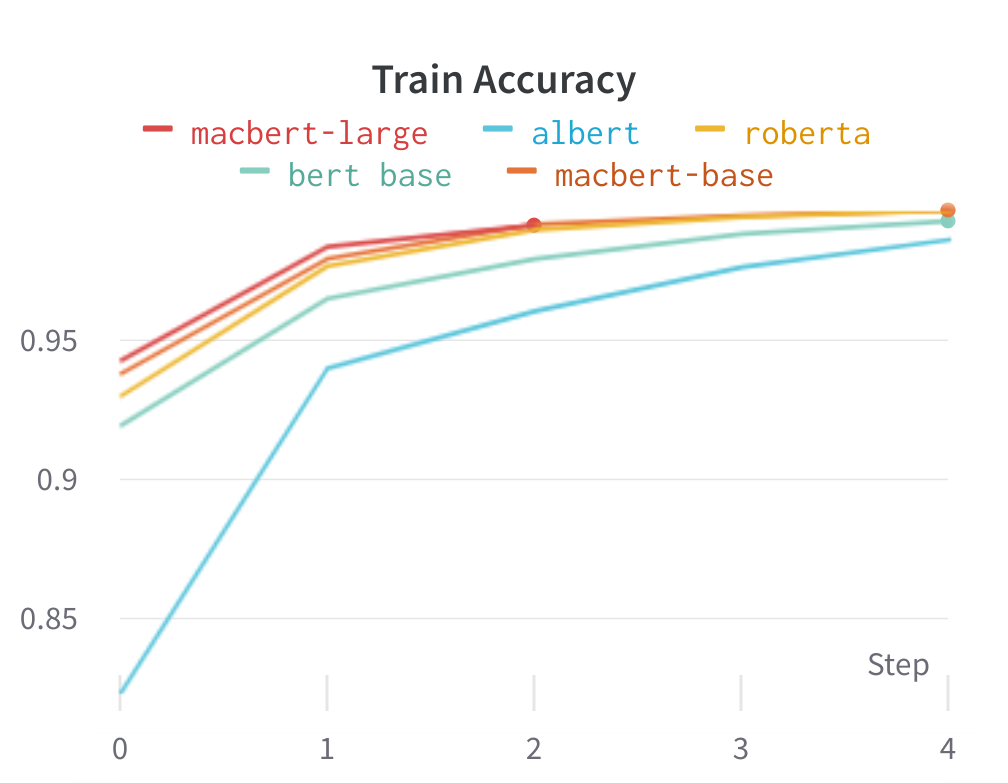
\includegraphics[width=\linewidth]{charts/Section-7-Panel-0-2whhfdmbm}
\endminipage\hfill
\minipage{0.49\textwidth}
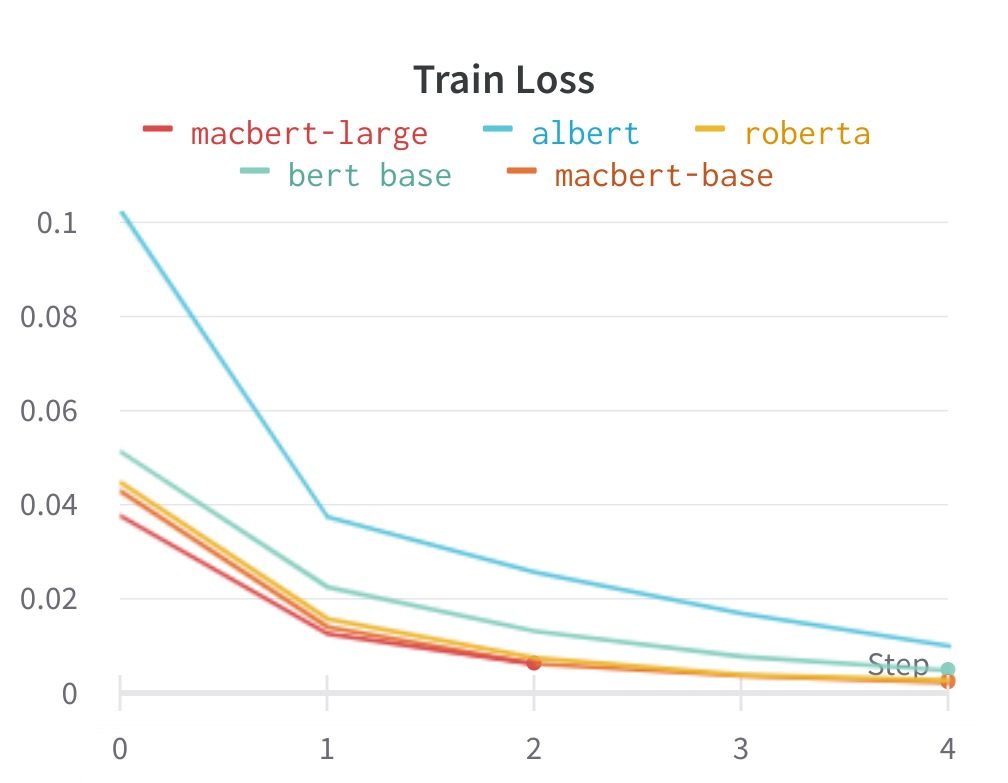
\includegraphics[width=\linewidth]{charts/Section-7-Panel-1-f1x11cdy7}
\endminipage
\end{figure}

\begin{figure}[!htb]
\minipage{0.49\textwidth}
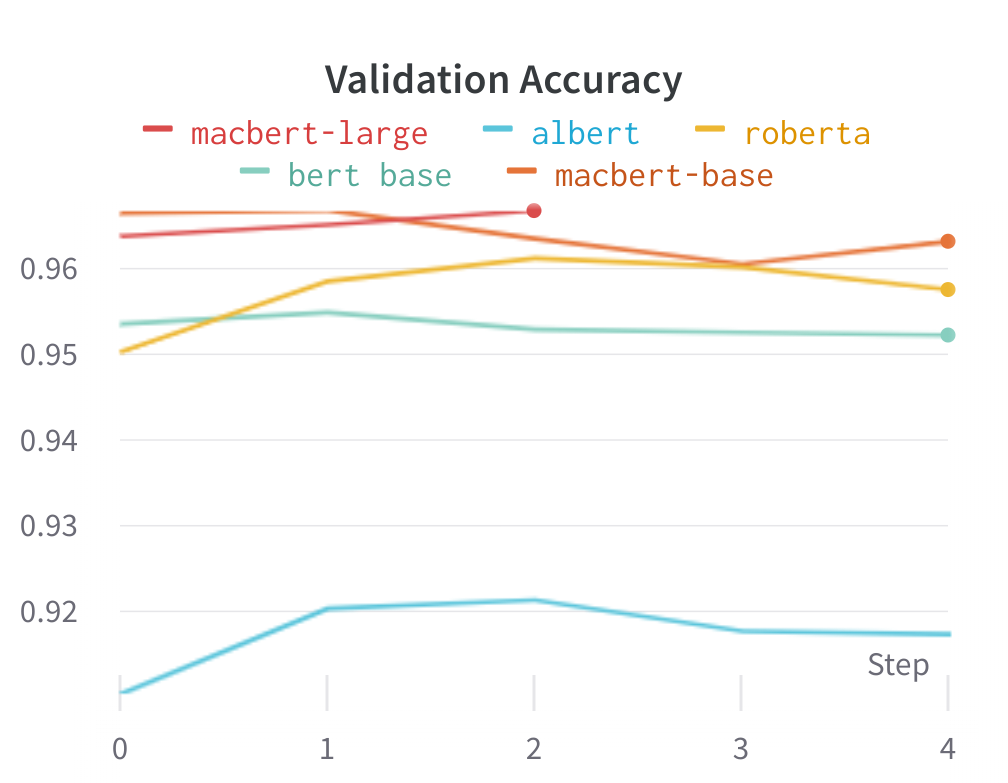
\includegraphics[width=\linewidth]{charts/Section-7-Panel-2-po8yi2tav}
\endminipage\hfill
\minipage{0.49\textwidth}
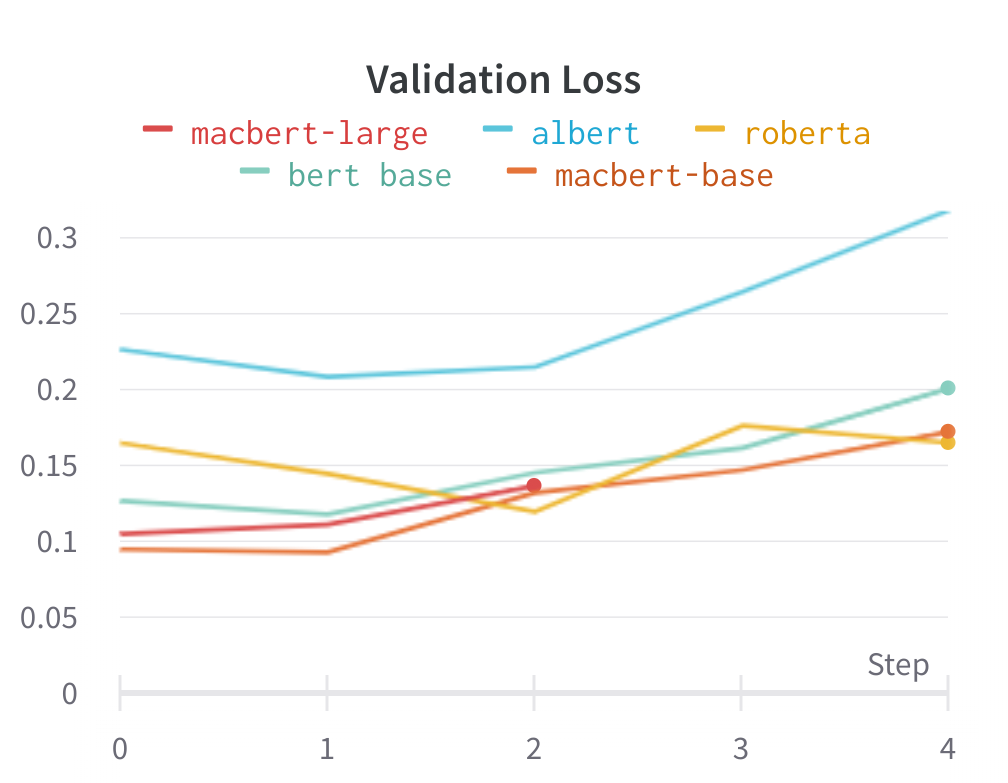
\includegraphics[width=\linewidth]{charts/Section-7-Panel-3-w0h4uy3ed}
\endminipage
\end{figure}
\clearpage
\subsection{Question Answering}
\begin{figure}[!htb]
\minipage{0.49\textwidth}
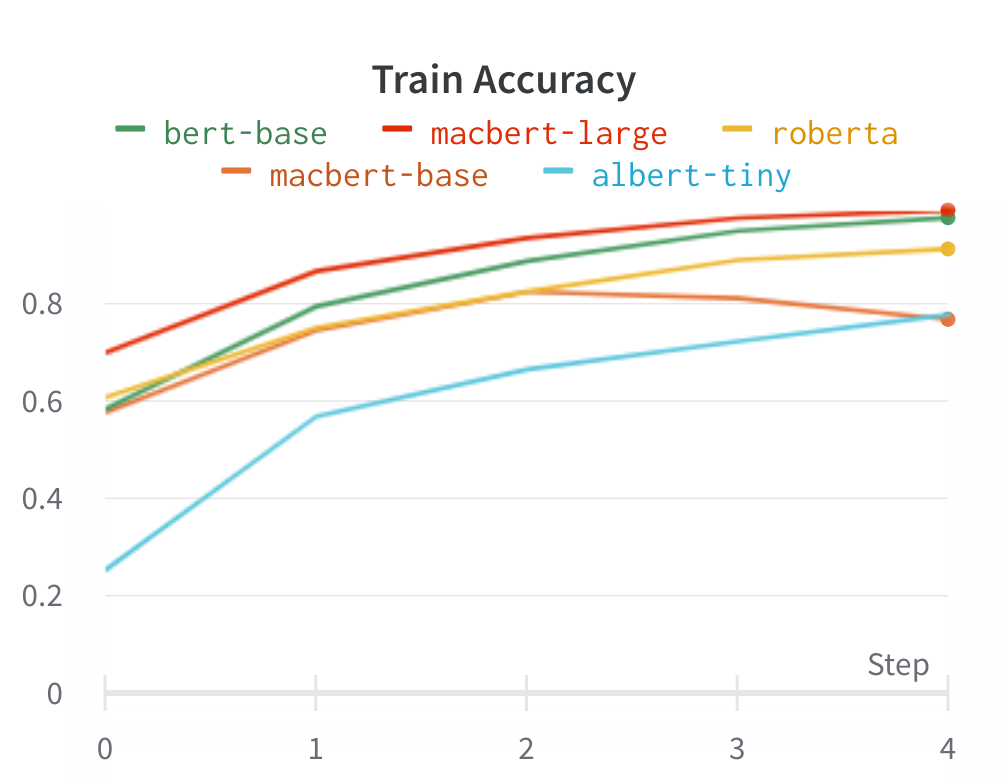
\includegraphics[width=\linewidth]{charts/Section-9-Panel-0-ic193coho}

\endminipage\hfill
\minipage{0.49\textwidth}
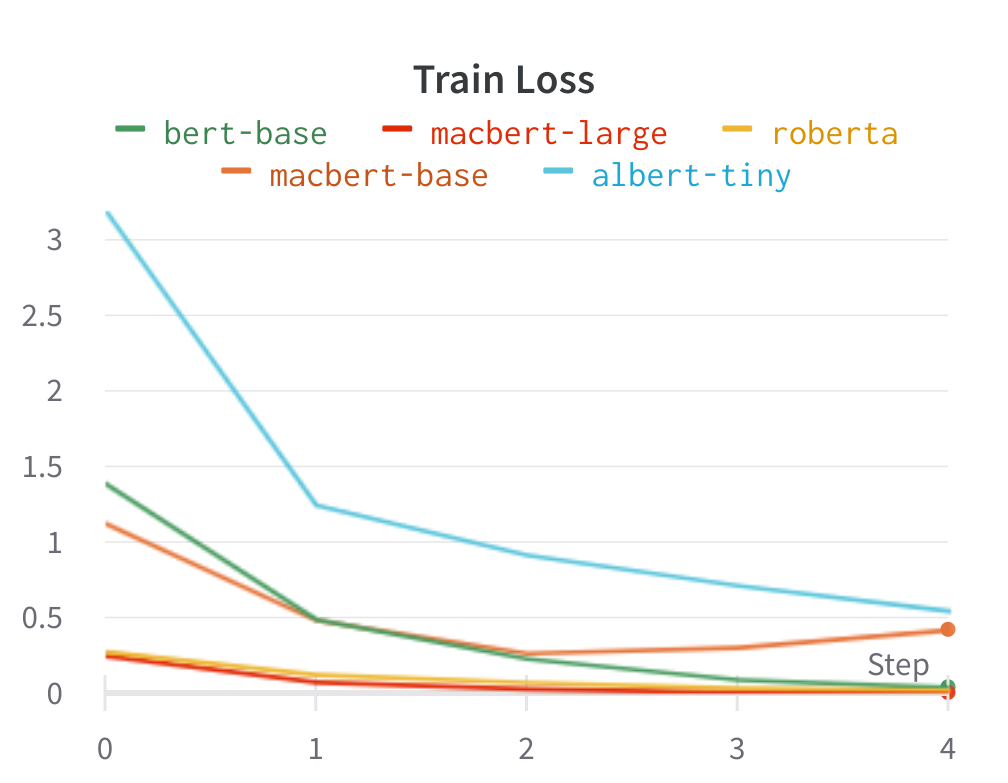
\includegraphics[width=\linewidth]{charts/Section-9-Panel-3-ssfbx70xn}

\endminipage
\end{figure}

\begin{figure}[!htb]
\minipage{0.49\textwidth}
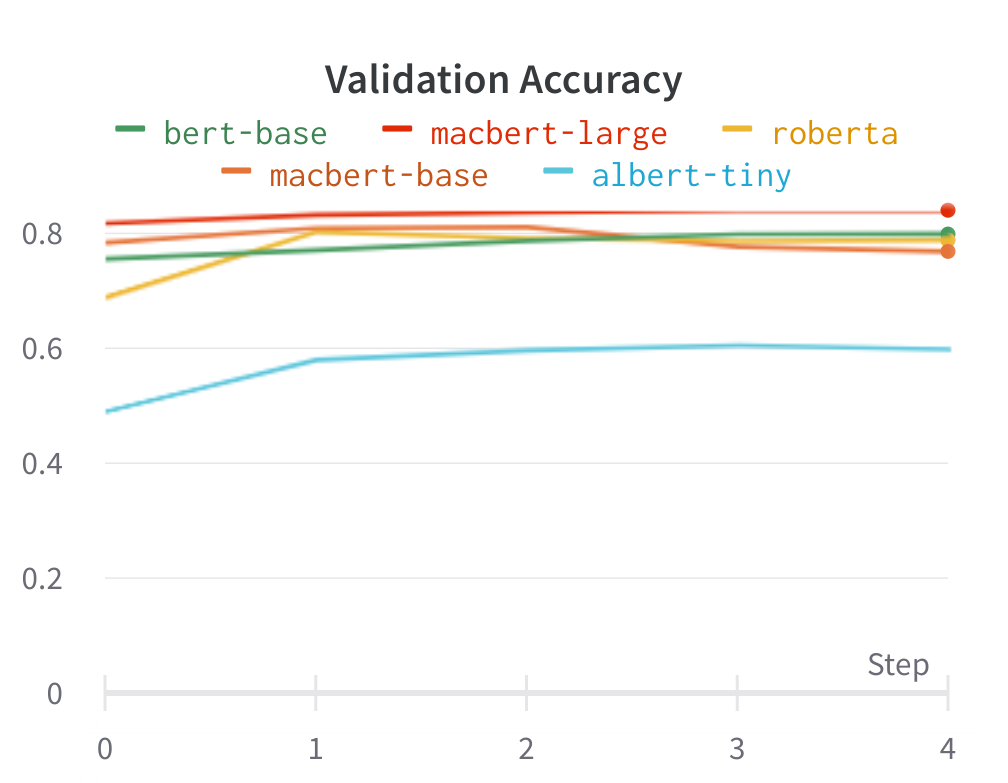
\includegraphics[width=\linewidth]{charts/Section-9-Panel-2-tjpy87ij0}

\endminipage\hfill
\minipage{0.49\textwidth}
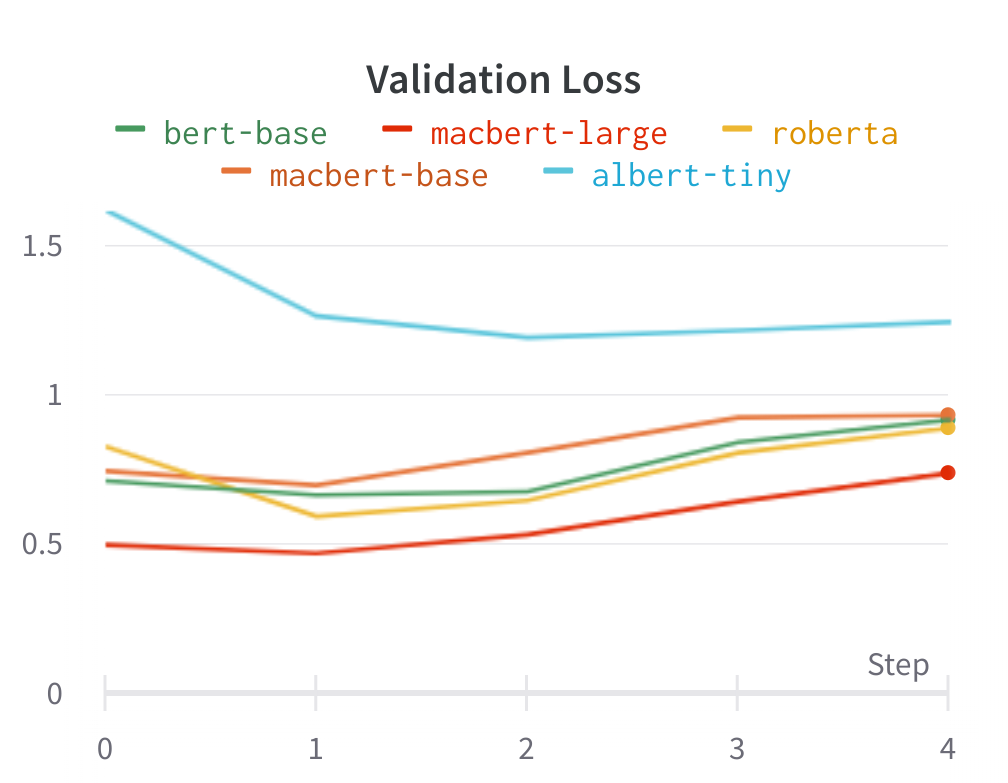
\includegraphics[width=\linewidth]{charts/Section-9-Panel-1-19njg3pxc}


\endminipage
\end{figure}
\newpage
\section{Pretrained vs From Scratch}
\subsection{Configuration}
The configuration on both tasks are the same.
Configuration:
\begin{itemize}
    \item Hidden size: 384
    \item Hidden Layers: 6
    \item Attention Heads: 6
    \item Intermediate Size: 1024
    \item \texttt{max\_len}: 384
    \item \texttt{doc\_stride}: 128
\end{itemize}
\subsection{Performance}
The best accuracy and the lowest loss are reported. \\
\begin{tabular}{c|c|c|c|c}
& Train Acc. / EM & Train Loss & Val. Acc. / EM & Val. Loss \\ 
\hline Context Selection & 0.9681 & 0.0534 & 0.35& 3.61 \\
\hline Question Answering & 0.9961 & 0.0170 & 0.54 & 0.9092 
\end{tabular}
\subsection{Comparison}
The model was trained from scrtach by simply removing the process of loading pretrained weight, who fits well on the training set but appears to be overfitting after around the tenth epoch on context selection task, and the weird thing is that the validation loss has been increasing since the first epoch from the first epoch to the last one in question answering. I thought this BERT was small enough but it still overfits, so I tried a smaller one with the following configuration, but the result is quite the same. 
\subsubsection{Even smaller BERT}
\begin{itemize}
    \item Hidden size: 256
    \item Hidden Layers: 4
    \item Attention Heads: 2
    \item Intermediate Size: 512
    \item \texttt{max\_len}: 256
    \item \texttt{doc\_stride}: 64
\end{itemize}
\newpage
\section{HW1 with BERTs}
\subsection{Model}
I used the widely-used RoBERTa (\texttt{roberta-base}) pretrained on pretrained on wikipedia and bookcorpus with the following configuration.
\subsubsection{Configuration}
\begin{itemize}
    \item Hidden size: 768
    \item Hidden Layers: 12
    \item Attention Heads: 12
    \item Intermediate Size: 3072
    \item \texttt{max\_len}: 512
\end{itemize}
\subsection{Performance}
The metrics reported are captured from the last epoch which is also the best. I didn't save the fine-tuned model so its performance on test dataset is not reported.
\subsubsection{Intent Classification}
\begin{tabular}{c|c|c|c|c}
    & Train Acc.  & Train Loss & Val. Acc.  & Val. Loss \\ \hline
    HW1 & 0.9942 & 0.01793 & 0.9332 & 0.7642 \\ 
    \hline  Transformer & 0.9887 & 0.1387 &  0.9701 & 0.1743
\end{tabular}
\subsubsection{Slog Tagging}
\begin{tabular}{c|c|c|c|c}
    & Train Acc.  & Train Loss & Val. Acc.  & Val. Loss \\ \hline
    HW1 & 0.955 & 0.001362 & 0.838 & 0.01562
     \\ 
    \hline  Transformer & 0.8096 & 0.0071 & 0.8290 & 0.0073
\end{tabular}
\subsection{Loss Function}
I used cross entropy loss for these two tasks.
\subsection{Optimization}
Exactly same setting as previously mentioned, AdamW optimizer with learning rate of $3\times 10^{-5}$ and weight decay of $1\times 10^{-6}$ and the same cosine scheduler with warmup.
\end{document}